\section{并行编程和计算思维}
到目前为止,我们专注于并行编程的实践知识,包括 CUDA 编程接口特性、GPU 架构、性能优化技术、并行模式和应用案例研究。 
在本章中,我们将讨论转向更抽象的概念。 
我们将并行编程的计算思维过程概括为:设计或选择并行算法,并将领域问题分解为明确定义和协调的工作单元。
每个工作单元都可以由所选算法有效地执行。 
具有强大计算思维能力的程序员不仅可以分析领域问题的结构,还可以转换领域问题的结构:哪些部分本质上是串行的,
哪些部分适合高性能并行执行,以及将部分从 前者为后者。 
通过良好的算法选择和问题分解,程序员可以在并行性、工作效率和资源消耗之间实现适当的折衷。 
为具有挑战性的领域问题创建成功的计算解决方案通常需要领域知识和计算思维技能的强有力结合。 
本章将使读者更深入地了解并行编程和通用计算思维。

\subsection{并行编程的目标}
在我们讨论并行编程的基本概念之前,我们首先回顾一下人们追求并行计算的三个主要原因。 
第一个目标是在更短的时间内解决给定的问题。 
例如,投资公司可能需要在交易后的时间里对其所有投资组合运行金融投资组合情景风险分析包。 
在顺序计算机上进行这样的分析可能需要 200 个小时。 
然而,投资组合管理流程可能要求在 4 小时内完成分析,以便根据结果信息及时做出重大决策。 
使用并行计算可以加快分析速度并使其在所需的时间窗口内完成。

使用并行计算的第二个目标是在给定的时间内解决更大的问题。 
在我们的金融投资组合分析示例中,投资公司可能能够使用顺序计算在给定时间窗口内对其当前投资组合运行投资组合情景风险分析。 
然而,该公司正计划扩大其投资组合中的持股数量。 扩大的问题规模会导致顺序分析超出允许的时间窗口。 
并行计算可以减少较大问题规模的运行时间,有助于适应计划的产品组合扩展。

使用并行计算的第三个目标是在给定的时间内为给定的问题获得更好的解决方案。 
投资公司可能在其投资组合情景风险分析中使用了近似模型。 
使用更准确的模型可能会增加计算复杂性并增加顺序计算机上的运行时间超出允许的窗口。 
例如,更准确的模型可能需要使用数字更复杂的公式来考虑更多类型的风险因素之间的相互作用。 
并行计算减少了更准确模型的运行时间,可以在允许的时间窗口内完成分析。

在实践中,并行计算可能是由这三个目标的组合驱动的。

从我们的讨论中可以清楚地看出,并行计算的主要动机是提高速度。 
第一个目标是通过提高在当前问题规模上运行现有模型的速度来实现的。 
第二个目标是通过提高现有模型在更大问题规模上的运行速度来实现的。 
第三个目标是通过提高在当前问题规模上运行更复杂模型的速度来实现的。 
显然,通过并行计算提高的速度可以用来实现这些目标的组合。 
例如,并行计算可以减少较大问题规模上更复杂模型的运行时间。

从我们的讨论中还应该清楚的是,适合并行计算的应用程序通常涉及大问题规模和高复杂性。 
即,这些应用程序处理大量数据,在每次迭代中需要大量计算,和/或对数据执行多次迭代。 
不涉及大问题或不会产生高建模复杂性的应用程序往往会在短时间内完成,并且不会提供太多提高速度的动力。

\begin{figure}[H]
	\centering
	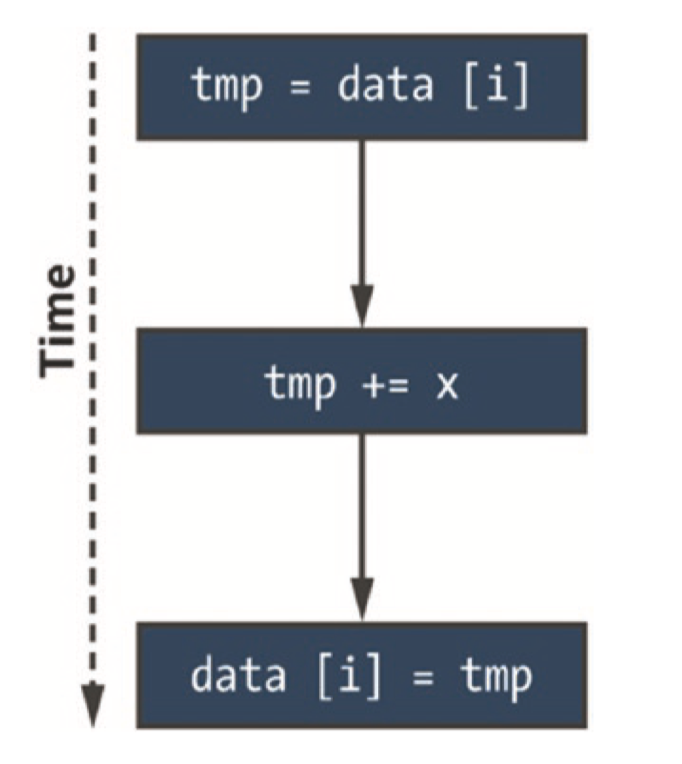
\includegraphics[width=0.9\textwidth]{figs/F19.1.png}
	\caption{\textit{分子动力学应用的主要任务。}}
\end{figure}

真实的应用程序通常由多个协同工作的模块组成。 图 19.1 显示了分子动力学应用程序主要模块的概述。 
对于系统中的每个原子,应用程序需要计算施加在原子上的各种形式的力,例如振动力、旋转力和非键合力。 
每种形式的力都用不同的方法计算。 在高层,程序员需要决定如何组织工作。 请注意,这些模块之间的工作量可能会有很大差异。 
非键合力计算通常涉及许多原子之间的相互作用,并且比振动力和旋转力需要更多的计算。 
因此,这些模块往往被实现为对力数据结构的单独传递。

程序员需要决定每个步骤是否值得在 CUDA 设备中实现。 
例如,程序员可能认为振动和旋转力计算不涉及足够的工作量来保证在 GPU 设备上执行。 
这样的决定将导致 CUDA 程序启动一个内核,计算所有网格点的非键合力场,同时继续计算主机上网格点的振动力和旋转力。 
更新原子位置和速度的模块也可以在主机上运行。 它首先结合来自主机的振动力和旋转力以及来自设备的非结合力。 
然后,它使用组合力来计算新的原子位置和速度。

设备完成的工作部分将最终决定整个应用程序能通过并行化获得多少加速。 
例如,假设非键合力计算占原始顺序执行时间的 95\%,并且使用 GPU 将其加速了 $100\times$。 
进一步假设应用程序的其余部分保留在主机上并且没有获得加速。 
应用程序级加速为 $1/(5\% + 95\%/100) = 1/(5\% + 0.95\%) = 1/(5.95\%) = 17\times$ 。 
在主机和CUDA设备的执行可以重叠的情况下,并行部分的执行时间完全隐藏在主机执行时间中。 
应用程序级加速将为 $1/(5\%) = 20\times$。这是阿姆达尔定律的演示:并行计算带来的应用程序加速受到应用程序的顺序部分的限制。 
在这种情况下,即使应用程序的连续部分非常小 (5\%),它仍将应用程序级别加速限制为 $20\times$ ,
尽管非键合力计算的加速比为 $100\times $ 并且完全隐藏在主机执行的阴影中。 
顺序部分。 此示例说明了加速大型应用程序的一个主要挑战:
不值得在 CUDA 设备上并行执行的小型活动的累积执行时间可能会成为最终用户看到的加速的限制因素。 
我们在第 17 章迭代磁共振成像重建的迭代 MRI 应用研究中看到了这种现象,
其中 CG 计算成为加速的限制因素,尽管它只占原始应用程序执行时间的 1\% 左右。

阿姆达尔定律经常促进任务级并行化。 尽管其中一些较小的活动不能保证细粒度的大规模并行执行,
但当数据集足够大时,可能需要彼此并行执行其中一些活动。 这可以通过使用多核主机并行执行此类任务来实现。 
或者,我们可以尝试同时执行多个小内核,每个小内核对应一个任务。 
CUDA 设备支持流的任务并行性,这将在第 20 章“异构计算集群编程”中讨论。

减少顺序任务影响的另一种方法是以分层方式利用数据并行性。 
例如,在消息传递接口(MPI,2009)实现中,分子动力学应用程序通常会将大块空间网格及其相关原子分发到网络计算集群的节点。 
通过使用每个节点的CPU来计算其原子块的振动力和旋转力,我们可以利用多个主机 CPU 并实现这些较小模块的加速。 
每个节点都可以使用 CUDA 设备以更高的加速水平计算非键合力。 节点需要交换数据以适应跨块的力和跨块边界移动的原子。 
我们将在第 20 章“异构计算集群编程”中讨论 MPI-CUDA 联合编程的更多细节。 
这里的要点是,MPI 和 CUDA 可以在应用程序中以互补、分层的方式使用,以共同实现大型数据集的更高速度。

并行编程的过程通常可以分为三个步骤:算法选择、问题分解以及性能优化和调优。 
最后一步是前几章的重点,并在第 6 章“性能注意事项”中进行了通用处理。 
在本章接下来的两节中,我们将普遍性和深度地讨论前两个步骤。

\subsection{算法选择}
算法是一个逐步的过程,其中每个步骤都被精确地说明并且可以由计算机执行。 
算法必须表现出三个基本属性:确定性、有效可计算性和有限性。 
确定性是指每个步骤都被精确地表述; 对于要做什么,没有任何含糊之处。 
有效的可计算性是指每一步都可以由计算机来执行。 有限性意味着必须保证算法终止。

给定一个问题,人们通常可以想出多种算法来解决该问题。 
有些比其他需要更少的计算步骤(即具有较低的算法复杂性),有些比其他具有更高程度的并行执行,有些比其他更普遍适用,
有些比其他具有更好的准确性或数值稳定性。 不幸的是,通常没有一种算法在所有这些方面都比其他算法更好。 
并行编程的程序员通常需要选择一种算法,以实现给定硬件系统的最佳折衷方案。

我们在本书的几个章节中看到了评估不同计算算法之间权衡的示例。 
对于第 11 章“前缀和(扫描)”中的前缀和计算,我们比较了执行并行前缀和的两种不同算法,
即 Kogge-Stone 算法和 Brent-Kung 算法。 我们的分析表明,Brent-Kung 算法具有较低的算法复杂度。 
执行相同的计算需要更少的操作,这使得工作效率更高。 
然而,我们还表明,Kogge-Stone 算法比 Brent-Kung 算法具有更多的并行性,使其能够以更少的迭代次数完成。 
算法复杂性和算法所表现的并行量之间的这种权衡是并行程序员遇到的典型权衡。 
最佳算法的通常取决于2个因素:目标硬件的并行特性和通过线程粗化把高复杂度的算法转换为高度并行算法或低复杂度顺序算法组合的能力。

对于第 13 章“排序”中的排序模式,我们比较了执行并行排序的两种不同算法,即基数排序和归并排序。 
基数排序可以实现比归并排序更低的算法复杂度,因为它是一种非比较排序算法。 它也非常适合并行化。 
然而,基数排序并不普遍适用,因为它只能与某些类型的键一起使用。 
归并排序是一种基于比较的排序,更普遍适用,并且可以与具有明确定义的比较运算符的任何类型的键一起使用。 
通用性和并行执行效率之间的权衡是并行程序员在选择并行算法时遇到的另一个权衡。

对于第 18 章“静电势图”中的静电势图计算,我们比较了执行计算的两种不同算法,
即直接库仑求和 (DCS) 和截止求和 (Rodrigues et al., 2008)。 
这两种方法具有相同程度的并行性并具有相同水平的通用性; 然而,它们提出了算法复杂性和准确性之间的经典权衡。 
在第18章“静电势图”中,我们证明了截止求和算法可以通过牺牲少量的精度来显着提高网格计算的执行效率。 
该技术解决的挑战是,通过完全精确的方法(例如 DCS)执行的计算量随着体积的平方而增加。 
对于大容量系统,这种增加使得计算时间过长,即使对于大规模并行设备也是如此。 
截止求和方法基于这样的观察:许多网格计算问题都基于物理定律,其中远离网格点的粒子或样本的数值贡献很小,
并且可以用隐式方法以低得多的算法来集中处理 复杂。 
尽管算法复杂性和准确性之间的这种权衡并不是并行编程所独有的,并且在顺序实现中也会遇到,但它可能会给并行程序员带来额外的挑战。 
我们在本节的其余部分中展示了截止求和算法的这些额外挑战的示例。

在顺序计算中,一种简单的截止算法一次处理一个原子。 对于每个原子,算法都会迭代位于原子坐标半径内的网格点。 
这是一个简单的过程,因为网格点位于一个数组中,可以轻松地将其索引为其坐标的函数。 然而,这个简单的过程并不容易并行执行。 
原因是,由于其分散的内存访问行为,以原子为中心的分解效果不佳。 
因此,我们需要使用一种基于网格中心分解的截止分箱算法:每个线程计算一个网格点的能量值。 
该算法的关键思想是首先根据输入原子的坐标将其分类到箱子中。 
每个箱子对应于网格空间中的一个方形区域,并包含坐标落入该方形区域的所有原子。 
我们将网格点的箱子的“邻域”定义为包含可以对网格点的能量值做出贡献的所有原子的箱子的集合。 
我们在第 18 章“静电势图”中描述了一种管理所有网格点邻域箱的有效方法。 
在此算法中,所有块都会迭代它们自己的邻域箱,而块中的所有线程一起扫描这些邻域箱中的原子,
但对每个原子是否落在其截止半径内做出单独的决定。

分箱的一个微妙问题是分箱最终可能含有不同数量的原子。 有些箱子可能有很多原子,有些箱子可能根本没有原子。 
一个众所周知的解决方案是将箱大小设置在合理的水平,通常远小于箱中原子的最大可能数量。分箱过程维护一个溢出列表。 
当原子被分类到容器中时,如果原子的主容器已满,则该原子将被添加到溢出列表中。 
在设备完成执行用于计算静电势图的截止求和内核之后,需要处理溢出列表中的原子以完成缺失的贡献。

\begin{figure}[H]
	\centering
	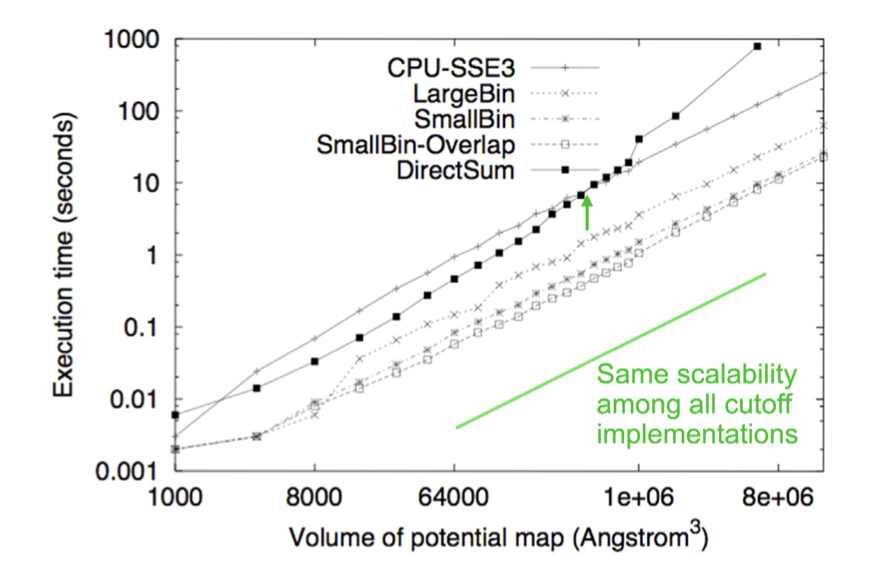
\includegraphics[width=0.9\textwidth]{figs/F19.2.png}
	\caption{\textit{DCS 与截止分级的可扩展性和性能。}}
\end{figure}

图 19.2 显示了各种静电势图算法和实现的可扩展性和性能的比较。 请注意,CPUSSE3 曲线基于顺序截止求和算法。 
对于体积较小的地图(大约 1000 A ),主机(带有 SSE 的 CPU)执行速度比 DCS 内核更快,如图 19.2 所示。 
这是因为对于如此小的体积,没有足够的工作来充分利用 CUDA 设备。 
然而,对于中等规模(2000 到 500,000 A 之间),由于其大规模并行性,直接求和内核的性能明显优于主机。 
然而,正如我们预期的那样,当卷大小达到约 1,000,000 A 时,直接求和内核的扩展性很差,并且运行时间比在 CPU 上的顺序算法更长! 
这是因为DCS内核的算法复杂度高于顺序截止算法,因此内核完成的工作量增长速度比顺序算法快得多。 
对于大于 1,000,000 A 的卷大小,工作量非常大,以至于会占用硬件执行资源。

图 19.2 还显示了截止求和算法的三种基于分箱实现的运行时间。 
SmallBin 实现对应于第 18 章静电势图中讨论的邻域 箱子 列表方法,并允许运行相同内核的块处理不同的原子邻域。 
SmallBin 实现确实会产生更多的指令开销,用于将原子从全局内存加载到共享内存中。 
对于中等体积,整个系统中的原子数量有限。 检查较少数量原子的能力并不能提供足够的优势来克服额外的指令开销。 
SmallBin-Overlap 实现将顺序溢出原子处理与下一个内核执行重叠。 
与 SmallBin 实现相比,它在运行时间方面提供了轻微但显着的改进。 
SmallBin-Overlap 实现比有效实现的顺序 CPU-SSE 截止求和实现实现了 $17\times$ 倍的加速,
并针对大容量保持了相同的可扩展性。

\subsection{问题分解}
选择合适的算法后,对于要通过并行计算解决的问题,必须以可以将其分解为可以同时安全解决的子问题的方式来表述。 
在这样的表述和分解下,程序员编写代码并组织数据来同时解决这些子问题。 
在大型计算问题中寻找并行性在概念上通常很简单,但在实践中可能具有挑战性。 
关键是要确定并行执行的每个单元要执行的工作,以便很好地利用问题固有的并行性。

\begin{figure}[H]
	\centering
	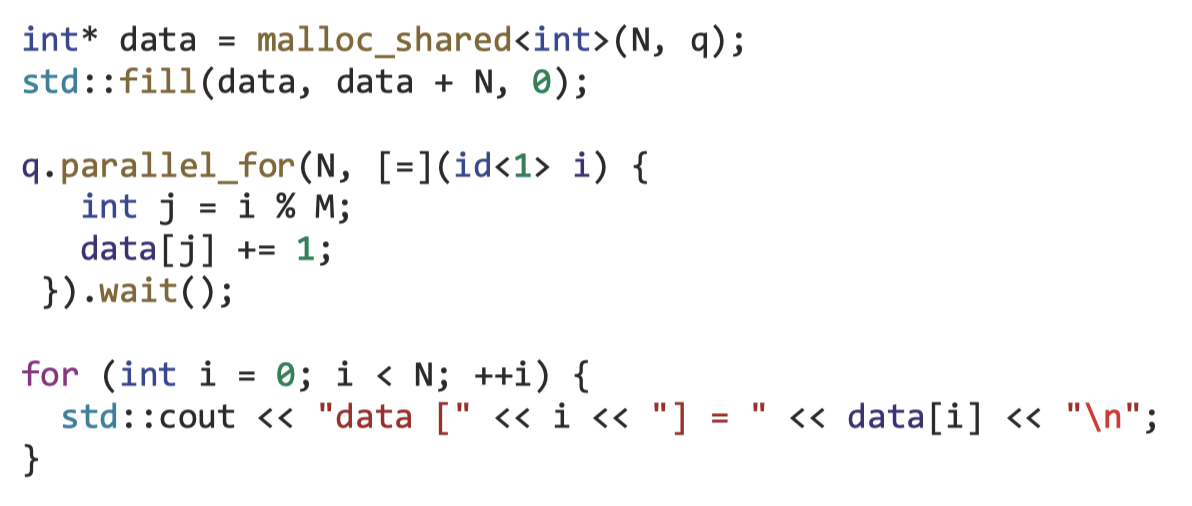
\includegraphics[width=0.9\textwidth]{figs/F19.3.png}
	\caption{\textit{问题分解策略。 (一)以输出为中心。 (B) 以输入为中心。}}
\end{figure}

分解并行执行问题的两种最常见的策略是以输出为中心和以输入为中心的分解。 
顾名思义,以输出为中心的分解分配线程来并行处理不同的输出数据单元,而以输入为中心的分解分配线程来并行处理不同的输入数据单元。 
这些分解策略如图 19.3 所示。 虽然两种分解策略都会产生相同的执行结果,但它们在给定的硬件系统中可能表现出截然不同的性能。 
以输出为中心的分解通常表现出收集内存访问行为,其中每个线程收集或收集输入值的影响到输出值。 
图 19.3A 说明了收集访问行为。 基于收集的访问模式在 CUDA 设备中通常更理想,因为线程可以将其结果累积在其私有寄存器中。 
此外,多个线程可以共享输入值,并且可以有效地使用常量内存缓存或共享内存来节省全局内存带宽。

相比之下,以输入为中心的分解通常表现出分散内存访问行为,其中每个线程将输入值的影响分散或分布到输出值中。 
散射行为如图 19.3B 所示。 基于分散的访问模式在 CUDA 设备中通常是不受欢迎的,因为多个线程可以同时更新同一网格点。 
网格点必须存储在可由所有涉及的线程写入的存储器中。 必须使用原子操作来防止多个线程同时写入输出值期间的竞争条件和值丢失。 
这些原子操作比以输出为中心的分解中使用的寄存器访问慢得多。

然而,除了聚集与分散访问模式之外,在决定以输出为中心还是以输入为中心的分解(或另一种分解)是否更适合特定应用程序时还可能需要考虑其他因素。 
这些考虑因素包括分解所暴露的并行性数量、识别哪些输入数据对哪些输出数据有贡献的容易程度、分解引起的负载平衡等,具体取决于应用程序。

以输入为中心和以输出为中心的分解之间的区别在第 17 章“迭代磁共振成像重建”和第 18 章“静电势图”中最为明显,
其中两种策略均得到实施并明确比较。 然而,问题分解是一个隐含的设计决策,在本书讨论的许多计算中都已做出。 
我们重新审视这些计算,以强调在每种情况下选择的问题分解以及为什么它比其他分解更有优势。

图像处理(第 3 章,多维网格和数据)、矩阵乘法(第 3、5 和 6 章)、卷积(第 7 章)和模板(第 8 章)计算均通过使用以输出为中心的分解来并行化。 
也就是说,这些计算中的线程被分配给输出元素(图像像素、矩阵条目或网格点),并迭代对它们有贡献的输入元素。 
或者,以输入为中心的分解会将线程分配给输入元素,并让每个线程迭代其输入元素所贡献的输出元素,并使用原子操作进行更新。 
在这些情况下,以输出为中心的分解相对于以输入为中心的分解的明显优势是通过使用聚集访问模式而不是分散访问模式来避免原子性。 
另一方面,其他考虑因素都没有使以输入为中心的分解有利。 
有足够的输出元素来展现高度的并行性,识别每个输出元素需要哪些输入元素非常简单,
并且所有输出元素需要相同的计算量,因此不存在负载不平衡。

直方图计算(第 9 章,并行直方图)通过使用以输入为中心的分解来并行化。 
也就是说,每个线程被分配给一个输入元素(或元素块)并根据输入值更新输出箱。 
由于多个线程可能会更新同一个输出仓,因此需要原子操作(分散访问模式)。 或
者,以输出为中心的分解会将线程分配给输出箱,并让每个线程搜索映射到箱的输入并相应地更新箱。 
这种分解将消除原子操作,因为每个容器将由单个线程更新(收集访问模式)。 
然而,以产出为中心的分解会产生许多其他问题。 首先,输出箱的数量通常远小于输入值的数量,因此并行性大大降低。 
其次,如果不检查这些输入值,线程就无法知道哪些输入值映射到其输出箱,因此每个线程都需要迭代每个输入值,这工作效率不高。 
第三,即使线程有某种方法可以快速识别哪些输入值映射到其输出箱,
每个箱也会有不同数量的输入值映射到它,这将在线程之间造成负载不平衡。 所有这些考虑使得以输入为中心的分解更有利于直方图计算。

合并操作(第 12 章,合并)通过使用以输出为中心的分解来并行化; 
也就是说,每个线程被分配给输出数组中的一个元素(或元素块),并执行二分搜索以查找相应的输入元素并将它们合并。 
虽然许多其他支持以输出为中心的分解的计算这样做是因为聚集相对于分散的好处,但这种考虑与合并操作无关。 
合并操作中的每个输出元素仅由一个输入元素贡献,因此以输入为中心的合并操作不需要使用原子。 
然而,以输入为中心的合并操作要么会使查找线程负责的输入元素与相应的输出元素之间的映射变得更加昂贵,
要么会因每个输入线程都具有高负载不平衡而导致负载不平衡。 负责不同数量的输入元素。 因此,优选以输出为中心的分解。

对于稀疏矩阵计算(第 14 章,稀疏矩阵计算),SpMV/COO 内核使用以输入为中心的分解,其中线程被分配给输入矩阵中的非零值,
并自动更新输出向量中的相应元素(分散访问模式)。 
其余内核使用以输出为中心的分解,其中线程被分配给输出向量元素并迭代输入非零(收集访问模式)。 
尽管以输入为中心的 SpMV/COO 内核执行原子操作,但与以输出为中心的内核相比,它具有其他优势,
例如提取更多并行性并具有更好的负载平衡。 最终,此计算的最佳分解取决于输入数据集。 
此外,混合 ELL-COO 格式展示了一个示例,其中以输出为中心和以输入为中心的混合分解可能是有益的。

对于图遍历(第 15 章,图遍历),以顶点为中心的推送实现和以边为中心的实现使用以输入为中心的分解。 
也就是说,线程被分配给顶点或边并更新相邻顶点的级别。 
相反,以顶点为中心的收集实现使用以输出为中心的分解,其中每个线程仅更新其分配到的顶点的级别。 
在不同的分解之间进行选择时,分散和聚集访问模式之间的权衡不是一个问题,因为对级别值的更新是幂等的并且不需要原子。 
然而,提取的并行量和实现的负载平衡在决定哪种分解更有利方面起着重要作用,并且最佳分解最终取决于输入数据集。 
我们鼓励读者回顾第 15 章“图遍历”,以更详细地处理该主题。

迭代 MRI 重建问题(第 17 章,迭代磁共振成像重建)和静电势计算问题(第 18 章,静电势图)都倾向于以输出为中心的分解,
因为与分散模式的聚集模式相比,它有利于避免 原子操作。 这些章节已经深入讨论了两种分解策略之间的区别。 
迭代MRI重建问题(第17章,迭代磁共振成像重建)处理大量的k空间样本数据。 
每个k空间样本数据也被多次用于计算其对重建体素数据的贡献。 对于高分辨率重建,每个样本数据都会被多次使用。 
我们表明,MRI 重建中 FhD 问题的良好分解是以输出为中心的分解,形成子问题,每个子问题使用聚集策略计算 FhD 元素的值。

类似地,静电势计算问题(第18章,静电势图)涉及计算许多输入原子对大量输出网格点势能的贡献。 
现实的分子系统模型通常涉及至少数十万个原子和数百万个能量网格点。 
每个原子的静电荷信息在计算其对能量网格点的贡献时被多次使用。 
我们证明静电势图计算问题的分解可以以原子为中心(即以输入为中心)或以网格为中心(即以输出为中心)。 
在以原子为中心的分解中,每个线程负责计算一个原子对所有网格点的影响。 
相反,以网格为中心的分解使用每个线程来计算所有原子对网格点的影响。 
以网格为中心(即以输出为中心)的分解被证明更好,因为它使用更有利的收集访问模式。 两种分解所暴露的并行性数量就足够了。 
对于截止求和算法,通过使用分箱克服了以网格为中心的分解中将输入数据映射到输出数据的困难,
并且通过上一节中讨论的 Small箱子-Overlap 实现克服了分箱导致的负载不平衡 。

\subsection{计算思维}
计算思维可以说是并行应用程序开发最重要的方面(Wing,2006)。 
我们将计算思维定义为根据计算步骤和算法制定领域问题的思维过程。 
与任何其他思维过程和解决问题的技能一样,计算思维是一门艺术。 
正如我们在第一章引言中提到的,我们认为最好通过迭代方法来教授计算思维,让学生在实践经验和抽象概念之间来回切换。

有大量关于各种算法、问题分解和优化策略的文献,但这些文献可能很难理解。 全面介绍所有可用技术超出了本书的范围。 
我们讨论了每个算法、问题分解和优化步骤中具有广泛适用性的大量技术。 
虽然这些技术是使用 CUDA C 实现进行演示的,但它们可以帮助读者建立通用计算思维的基础。 
我们相信,当我们自下而上学习时,人类理解得最好。 
也就是说,我们首先在特定编程模型的上下文中学习概念,这为我们在将知识推广到其他编程模型之前提供了坚实的基础。 
对 CUDA C 实现的深入体验也使我们变得成熟,这将帮助我们学习甚至可能与 GPU 无关的并行编程和计算思维概念。

并行程序员要成为有效的计算思考者,需要具备多种技能。 我们将这些基本技能总结如下:
\begin{itemize}
	\item 计算机体系结构:内存组织、缓存和局部性、内存带宽、SIMT 与 SPMD 与 SIMD 执行以及浮点精度与准确度。 
		这些概念对于理解算法、问题分解和优化之间的权衡至关重要。

	\item 编程接口和编译器:并行执行模型、可用存储器类型、同步支持类型、数组数据布局和线程粒度转换。 
		需要这些概念来思考数据结构和循环结构的安排,以实现更好的性能。

	\item 领域知识:问题表述、硬约束与软约束、数值方法、精度、准确度和数值稳定性。 
		了解这些基本规则可以让开发人员在应用算法技术时更具创造性。
\end{itemize}

我们编写本书的目标是为所有这些领域提供坚实的基础。 读完本书后,读者应继续扩大这些领域的知识。 
最重要的是,培养更多计算思维技能的最佳方法是不断用优秀的计算解决方案解决具有挑战性的问题。

有效利用计算的一个良好目标是让科学变得更好,而不仅仅是更快。 
这需要重新审视先前的假设,并真正思考如何应用大规模并行处理的大锤。 
换句话说,“仅仅重新编译”或使用相同计算方法使用更多线程可能不会获得诺贝尔奖或图灵奖。
 真正重要的科学发现更有可能来自新的计算思维。 将此视为利用计算能力的巨大财富以新方式解决新问题的劝告。

攻克计算密集型应用程序的方法有三种,其难度、复杂性和回报潜力依次递增,这并不奇怪。 
让我们称这些为“好”、“更好”和“最好”。

“好”的方法就是“加速”遗留的程序代码。 
最基本的工作就是重新编译并在新的平台或架构上运行,而不添加任何并行领域的见解或专业知识。 
这可以通过使用优化的库、工具或指令来增强,例如 CuBLAS、CuFFT、Thrust、Matlab 或 OpenACC。 
这种方法不需要任何算法选择、问题分解或优化和调整工作。 
对于领域科学家来说,它可以立即带来回报,因为只需最少的计算机科学知识或编程技能即可获得相当大的加速。 
然而,它并没有充分发挥并行计算的潜力。

“更好”的方法涉及使用并行编程技能重写现有代码以利用新架构或从头开始创建新代码。 
这种方法是巧妙思考问题分解和优化选择的机会,对于非领域计算机科学家来说是一项很好的工作,因为只需要最少的领域知识。 
然而,由于缺乏有效算法选择所需的特定领域知识,它也没有充分发挥并行计算的潜力。

“最佳”方法涉及应用程序并行化的整体尝试,涉及所有三个关键步骤:算法选择、问题分解以及优化和调整。 
我们不仅希望将已知算法映射到并行程序并对其进行优化,而且希望重新思考解决方案中使用的数值方法和算法。 
第 18 章“静电势图”中的截止分箱方法就是一个很好的例子。 
该方法需要领域专业知识,以牺牲准确性来显着降低算法复杂性,并且需要问题分解和优化技能,
以将以网格为中心的分解与计算机科学家设计的分箱技术结合使用。 
通过这种方法,有可能获得最大的性能优势以及根本性的新发现和功能。 
例如,人们可能能够对生化系统进行高保真模拟,其规模被认为是传统方法无法达到的。 
这种方法是跨学科的,需要计算机科学和领域洞察力,但回报是值得的。 对于一名计算科学家来说,这确实是一个激动人心的时刻!

\subsection{总结}
综上所述,我们讨论了并行编程和计算思维的主要步骤,即算法选择、问题分解以及优化和调优。 
给定一个计算问题,程序员通常必须从多种算法中进行选择。 其中一些算法在保持相同数值精度的同时实现了不同的权衡。 
其他方法则涉及牺牲一定程度的准确性来实现更具可扩展性的运行时间。 
对于所选算法,问题分解的不同选择可能会导致线程之间不同程度的干扰、并行性暴露、负载不平衡以及并行执行期间的其他性能考虑。 
计算思维技能使算法设计者能够克服障碍并找到良好的解决方案。